\chapter{Asterisk, an open source PBX}

\section{Why Asterisk?}
For this project, we tried to look for an efficient telephony server. A server with a lot of documentation and a great community support would be ideal. Moreover, this server should be really flexible because the configuration will be often generated, and then reloaded.
Because lot of these PBX are managed by a web GUI interface, we discovered \textit{Asterisk}. It seemed to be the ideal server we needed. It have an excellent community support, a great documentation and able to reload its configuration fastly without interrupting current communications.

\section{Server compilation}
Because \textit{Asterisk} is provided as open source server, we had to download the server sources and then compile them with the following commands:
\begin{lstlisting}[language=bash,caption={bash}]
$ ./configure
$ make menuconfig
$ make
$ make install
\end{lstlisting}

One of the most important command in the above list was \textit{make menuselect}: this command allows to enable and disable unwanted modules. It is there we can enable for example the MP3 support.

\section{Server organization}

\subsection{Contexts}
On Asterisk, all phone activities are based on contexts. It means when a phone is registered in a context, it can't reach phones which are located in different context. The contexts will be mainly useful for the company switchboard. Indeed, all switchboard will have their own context called like \textbf{SWITCHBOARD\_USER\_(CODE)} where (CODE) is replaced by the switchboard access code, defined at the creation of the switchboard on the website.


\textit{ScotIP} purposes two kinds of lines: the dedicated line and the shared lines.
Shared lines will share the same starting context. This context is called \textbf{ScotIPHome}. It is a vocal service where all incoming calls will be redirected. This vocal service will ask the caller to enter the switchboard access code, and if it exists, then the caller will be redirected on the switchboard context.


This is possible thanks to variables, conditions and functions provided in Asterisk. When the caller will press his phone keys, the number will be stored in a temporary variable. Then, thanks to the function \textbf{DIALPLAN\_EXISTS(name)} the caller can be redirected on the right context. Otherwise, the call will be hang up. 


\begin{figure}[!ht]
  \caption{ScotIPHOME context.}
  \centering
    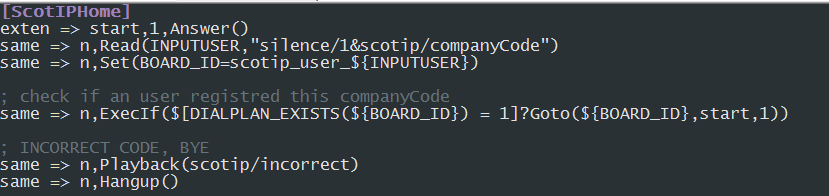
\includegraphics[width=0.5\textwidth]{img/context_scotiphome.png}
\end{figure}

\subsection{Files and \#include directive}

Because Asterisk configuration have to be located in \textit{/etc/asterisk} directory, the configuration can't be flexible. However, one directive exists to bypass this obligation. \textbf{\#include}. Thanks to this directive, we could organize our server architecture in many subdirectories. This directive allows also the use of \textit{jokers}, represented by this character: \textbf{*}. In our application, we chose to save all these files to the directory \textit{/usr/scotip}.

Each directory will match one type of configuration file. For example, we have to save the dialplans for the company switchboards, music on hold files, extensions configuration... 

\begin{figure}[!ht]
  \caption{Directory structure.}
  \centering
    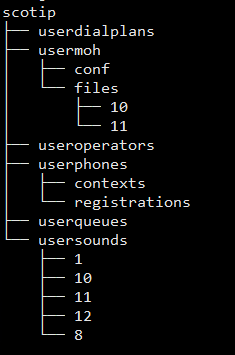
\includegraphics[width=0.5\textwidth]{img/files_struct_conf.png}
\end{figure}


\section{SIP}

\subsection{SIP communication}
Asterisk supports a lot of protocol but for this project, we only used the SIP protocol. It is why we will only talk about this one.
The SIP protocol is described by the \href{http://www.rfc-base.org/rfc-3261.html}{\textit{RFC 3261}}.


\begin{figure}[!ht]
  \caption{SIP callflow example. Source: Wikipedia}
  \centering
    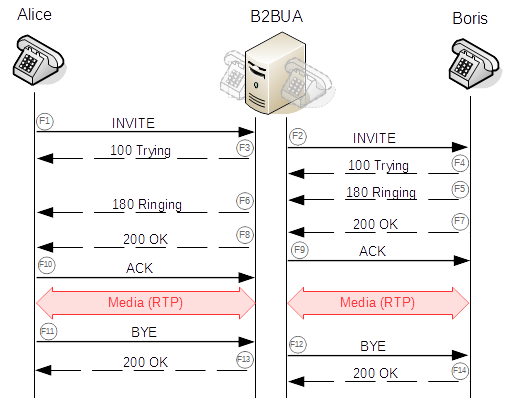
\includegraphics[width=1\textwidth]{img/callflow.png}
\end{figure}

\subsubsection{SIP request}
As SIP requests are simple, SIP requests are delivered over UDP protocol which don't need a persistent connection.  

\begin{itemize}
\item REGISTER: Used by a UA to register to the registrar.
\item INVITE: Used to establish a media session between user agents.
\item ACK: Confirms reliable message exchanges.
\item CANCEL: Terminates a pending request.
\item BYE: Terminates an existing session.
\item OPTIONS: Requests information about the capabilities of a caller without the need to set up a session. Often used as keepalive messages.
\item REFER: indicates that the recipient (identified by the Request-URI) should contact a third party using the contact information provided in the request. (call transfer)
\end{itemize}
\textit{\small{Source: Wikipedia and RFC}}


\subsubsection{SIP response}
As for the SIP requests, SIP responses are delivered over UDP protocol. The response only consists of a response code which means if the operation has been allowed or not. 

\begin{itemize}
\item Provisional (1xx): Request received and being processed.
\item Success (2xx): The action was successfully received, understood, and accepted.
\item Redirection (3xx): Further action needs to be taken (typically by sender) to complete the request.
\item Client Error (4xx): The request contains bad syntax or cannot be fulfilled at the server.
\item Server Error (5xx): The server failed to fulfill an apparently valid request.
\item Global Failure (6xx): The request cannot be fulfilled at any server.
\end{itemize}
\textit{\small{Source: Wikipedia and RFC}}




\subsubsection{RTP}
Once a communication is established between a SIP client and a server, when an ACK command has been sent by the server, a new connection is established between them through the RTP protocol. It is this protocol, described for the first time in \textit{RFC 1889} in 1996, which allows the audio and video delivering. 

 
\begin{figure}[!ht]
  \caption{RTP header.}
  \centering
    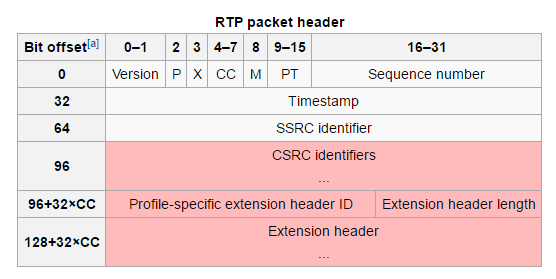
\includegraphics[width=1\textwidth]{img/rtpheader.png}
\end{figure}
\textit{\small{Source: Wikipedia \url{https://en.wikipedia.org/wiki/Real-time_Transport_Protocol}}}


\subsection{SIP peers}
In order to emit and receive calls, we have to register on the network on our providers. To use these networks, there are two important steps. 


First, we have to write a registration string of this kind: \textit{register => username:password@provider.dot.ltd}. This line allows to register our server to use the provider network. The state of this connection through the command line: \textit{sip show registry}

\begin{figure}[!ht]
  \caption{SIP registrations.}
  \centering
    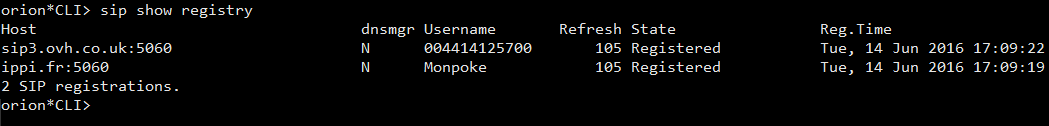
\includegraphics[width=1\textwidth]{img/sipshowregistry.png}
\end{figure}



For the second step, we have to tell Asterisk in which context the incoming calls have to be redirected, and also make some settings on the connection. (Eg: monitoring, incoming host...)
Because on our project we only made possible incoming calls, we will not talk about outgoing calls in this report. For all these calls, they will be redirected on a local context called \textbf{phone\_incoming}, then redirected on a global context for all the project: \textbf{ScotIPHome}, which have been previously described.

\begin{figure}[!ht]
  \caption{Incoming contexts.}
  \centering
    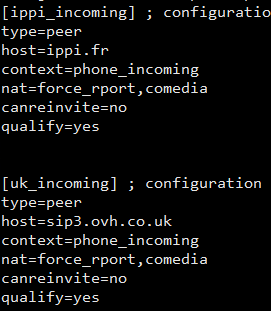
\includegraphics[width=0.5\textwidth]{img/contextsphones.png}
\end{figure}

\subsection{SIP accounts}


\subsection{Calling Skype account}
Because we couldn't afford a SIP line for Skype, thanks to our provider \textit{IPPI}, it becomes possible to emit calls to Skype. However, some configuration is still needed. Firstly, we have to register an outgoing context with IPPI.

\begin{figure}[!ht]
  \caption{Skype context.}
  \centering
    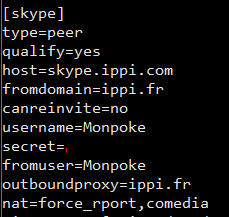
\includegraphics[width=0.5\textwidth]{img/skypeout.png}
\end{figure}

To call a Skype account, we just have to precise the account name then the context name: \textbf{mySkypeAccount@skype}. 


\textbf{@TODO}

\section{Switchboard, modules and extensions}
To represent a switchboard, we're using the extensions from \textit{Asterisk}. All these extensions have to be located in a context. For our project, all extensions related to a switchboard will be placed in the switchboard context we saw earlier: \textbf{SWITCHBOARD\_USER\_(CODE)}. \newline

On the home context, \textit{ScotIPHome}, when a right access code is entered, the caller is redirected on a first extension in the switchboard context, called \textit{start}.
All these switchboard context contains this first extension. This one sets some global variables which could be useful for the next extensions, like the current \textit{switchboard id}, the \textit{caller number}... \newline

\subsection{Modules extensions}

For our project, we have two types of extensions:
\begin{itemize}
\item \textbf{"Binding keys"}
\item \textbf{Extension for a module}
\end{itemize}

The second type corresponds to the chosen module. For each one, two variables are defined in order to be used later. The name of these extensions are called in this way: \textbf{SWITCHBOARD\_USER\_(CODE)}.
Afterwards, the Asterisk function is finally called.  We'll speak about these functions in next sections.





\section{Used Asterisk applications}
\subsection{Playback}
In Asterisk, one of the most used application is \textbf{Playback}. This command makes available the streaming of a file in a channel. 


\begin{lstlisting}[language=bash,caption={Syntax of application Playback}]
Playback(filename&[filename2[&...]],[options])
\end{lstlisting}

\subparagraph{Arguments}
\begin{itemize}

	\item filenames
	\begin{itemize}
		\item filename
		\item filename2
	\end{itemize}
	
	\item options - Comma separated list of options
		\begin{itemize}
		\item skip - Do not play if not answered
		\item noanswer - Playback without answering, otherwise the channel will be answered before the sound is played.
		\end{itemize}
\end{itemize}

\subparagraph{Usage in our project:}
For \textit{ScotIP}, we used this command to play audio files which cannot be skipped.  




\subsection{Read}
When you require the caller to type something, this command should be used. Based on the DTMF tone, the interpreted result is saved in a given variable. 


\begin{lstlisting}[language=bash,caption={Syntax of application Read}]
Read(variable,filename&[filename2[&...]],[maxdigits,[options,[attempts,[timeout]]]]])
\end{lstlisting}

\subparagraph{Arguments}
\begin{itemize}
	\item variable - The input digits will be stored in the given variable name
	\item filenames - Files will be read while waiting for input
	\begin{itemize}
		\item filename
		\item filename2
	\end{itemize}
	
	\item maxdigits - Maximum of digits
	\item options - Specify some options
	\item attempts - Do not play if not answered
	\item timeout - Wait for x seconds
\end{itemize}

\subparagraph{Usage in our project:}
This command has been often used. Because the previous application, \textit{Playback}, doesn't allow to be skipped, we used \textit{Dial} for this purpose. Indeed, because for each module, except the root module, the caller have to press a key to reach a next module, we can use this application. It will play specified file until a key is pressed. \newline

Furthermore, this application is also used for the module \textit{User input} on the website, and is used to get the code of the company which have to be reached on the welcome context (\textbf{ScotIPHome}). 


\subparagraph{About DTMF:}
\textit{Dual-tone multi-frequency signaling} (DTMF) is an in-band telecommunication signaling system using the voice-frequency band over telephone lines. 

\begin{figure}[!ht]
  \caption{DTMF frequencies.}
  \centering
    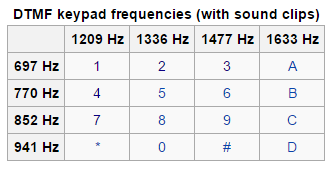
\includegraphics[width=0.5\textwidth]{img/dtmf.png}
\end{figure}

{\textit{Source:} Wikipedia} \url{https://en.wikipedia.org/wiki/Dual-tone_multi-frequency_signaling}
	


\subsection{Dial}
This application is also one of the most used. Dial is the application which try to establish a new connection between two channels. 



\begin{lstlisting}[language=bash,caption={Syntax of application Dial}]
Dial(technology/identifier1, timeout, options)
\end{lstlisting}

\subparagraph{Arguments}
\begin{itemize}

	\item technology/identifier1 - Precise the technology type (SIP/IAX2...) followed by an identifier. 
	\item timeout - Specify a ringing time before cancel the dial application
	\item options - Comma separated list of options (only used options listed)
	\begin{itemize}
		\item m(mohclass) - Specify some class of music on hold while ringing
	\end{itemize}
	
\end{itemize}

\subparagraph{Usage in our project:}
For \textit{ScotIP}, this application has been used to join operators. Because the operators was registered on the internal server, we could it as following: \textit{Dial(SIP/operator\_1,...)}. To contact a \textit{Skype} account, the call has to be forwarded through the context \textit{skype}, described previously. To use this context, the function becomes \textit{Dial(SIP/skypeUsername@skype,...)}.





\subsection{Queue}
\textbf{Queue} is an application really useful to welcome messages. For example, it is used to make wait callers when no operators is available to answer their call. While they are waiting, some music on hold can be played. 


\begin{lstlisting}[language=bash,caption={Syntax of application Playback}]
Queue(queuename,...)
\end{lstlisting}

\subparagraph{Arguments}
\begin{itemize}

	\item queuename - Contains the queue name where the caller should be added
\end{itemize}

\subparagraph{Usage in our project:}
For \textit{ScotIP}, we used this application for the company queues, created from the website.


\subsection{Macro}



\section{MOH}
\subsection{About}
\subsection{Conversion}
Not here, but in website 
